% % % % % % % % % % % % % % % % % % % % % % % % % % % % % % % % % % % % % % % % %
% INTRO
% % % % % % % % % % % % % % % % % % % % % % % % % % % % % % % % % % % % % % % % %
\section{Time box 7}
\listoftodos
\subsection{Time box planning}

\begin{figure}[H]
	\begin{centering}
		\missingfigure{Updated timebox figure}
		%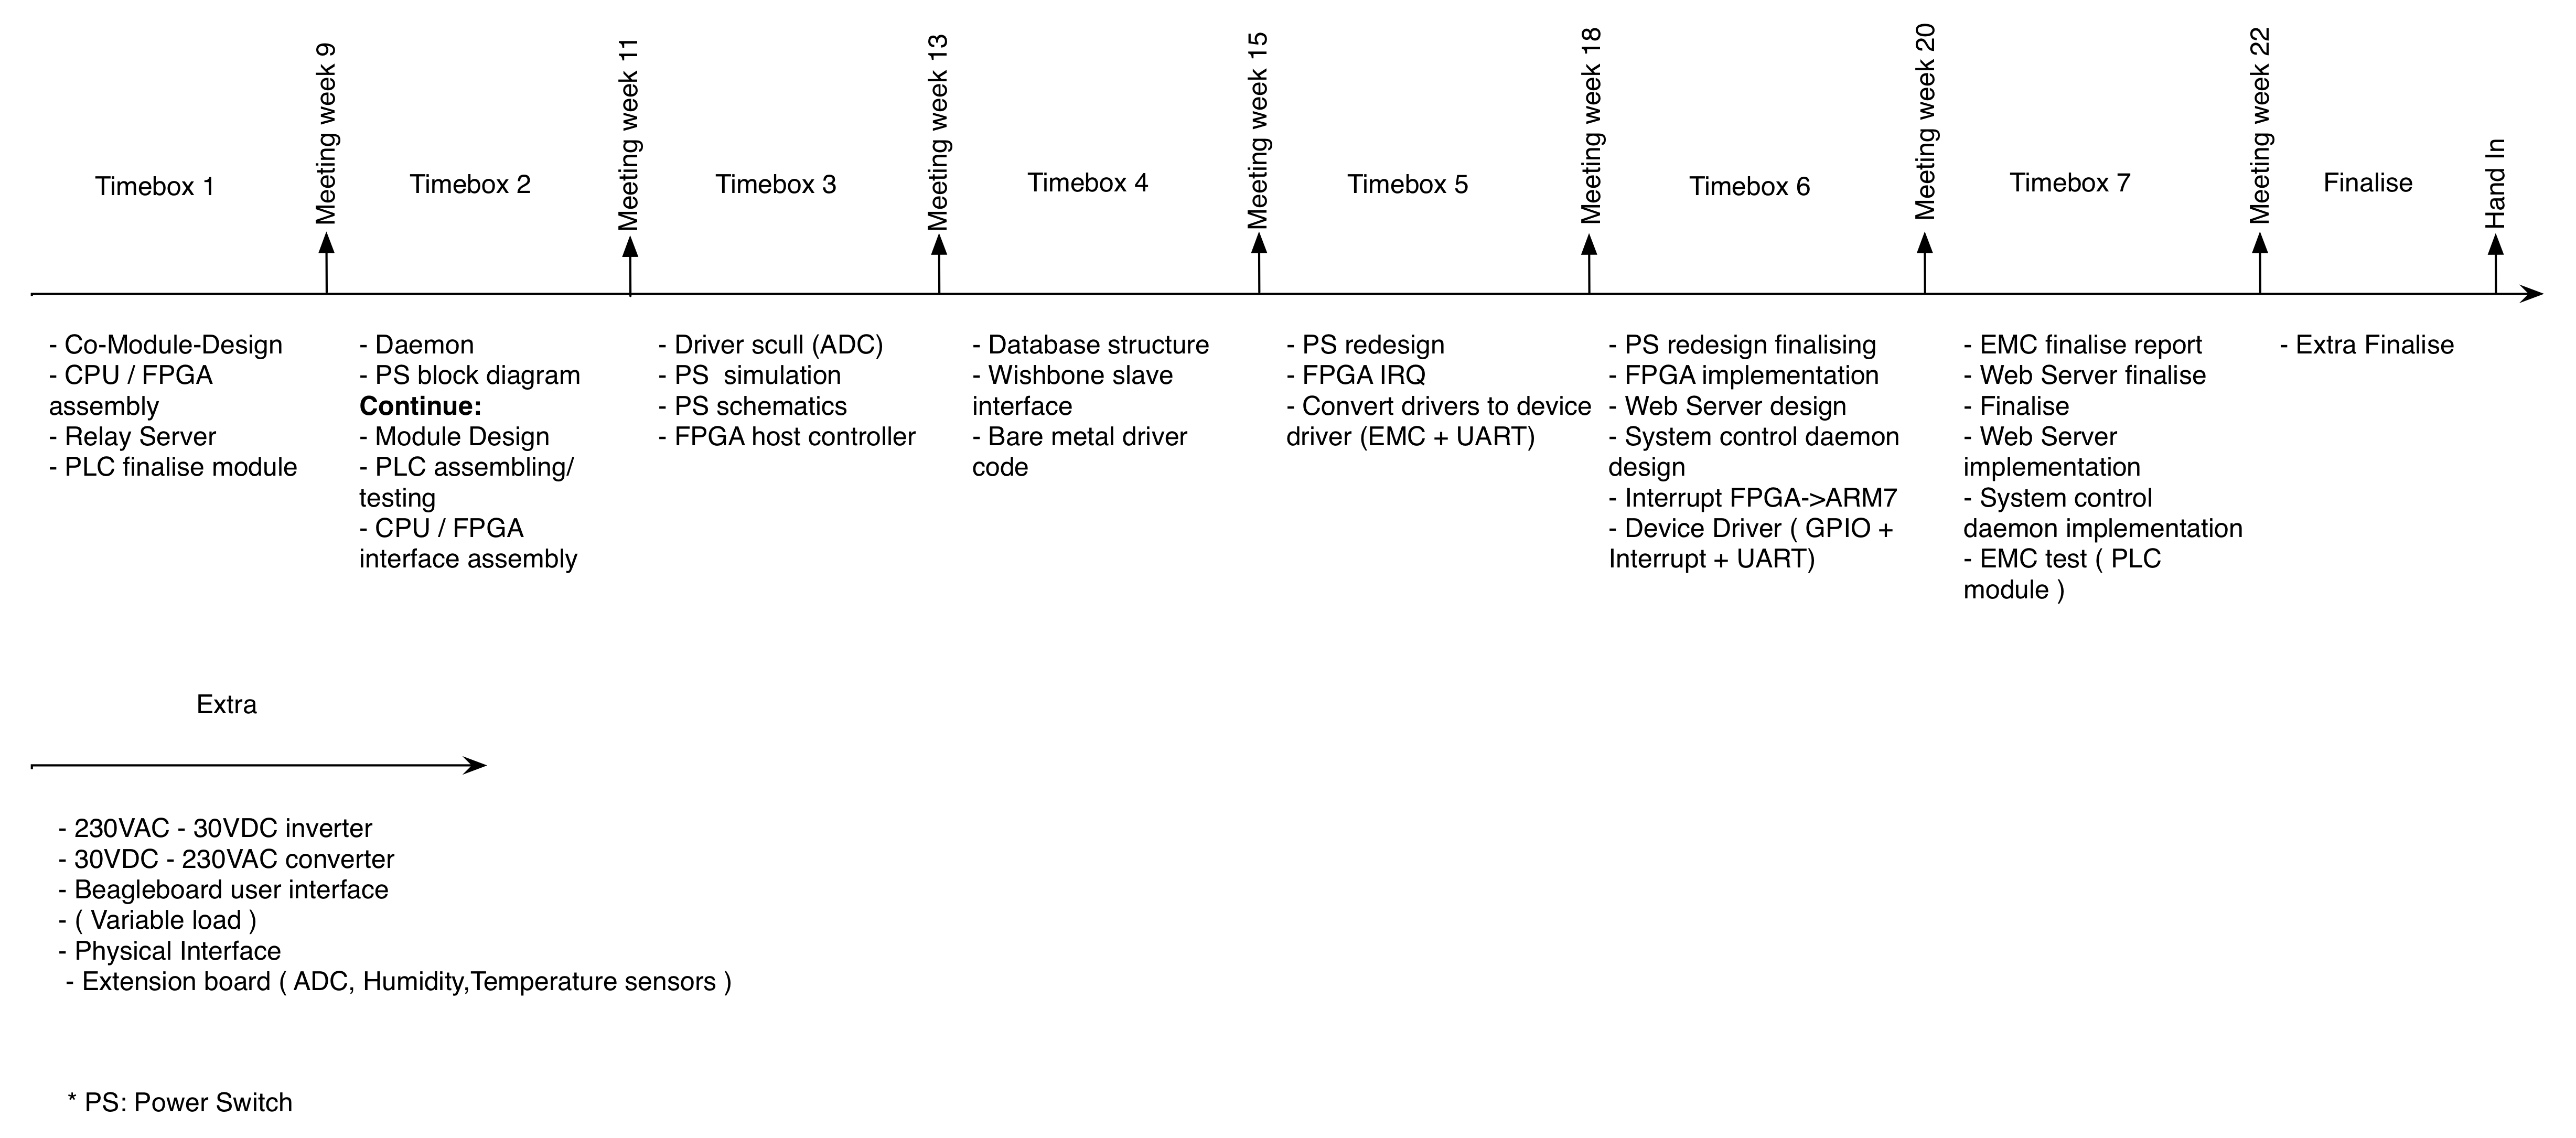
\includegraphics[width=1.0\textwidth]{images/tb_r5.png}
		%\caption{Updated time-box}
	\end{centering}
\end{figure}

\subsubsection{Work to be done in this time box}
\todo[inline]{Update List}
\begin{itemize}
	\item Requirements for debouncing
	\begin{itemize}
		\item Stability of switches
		\item Time limits
	\end{itemize}
	\item Verification
	\begin{itemize}
		\item External memory controller
		\item Verification of the Spartan 6
	\end{itemize}
	\item Jesus thing
		\begin{itemize}
			\item sub thing
		\end{itemize}
	\item GPIO Device driver
	\begin{itemize}
		\item Setup and control of GPIO pins used in the system
	\end{itemize}
\end{itemize}

\paragraph{Description:}
\todo[inline]{Update Description}
\begin{description}
	\item[Requirements for debouncing] This is the timing requirements for the switch block to avoid bouncing when switching state
	\item[Verification] This is verification of the VHDL design including the EMC part in the LPC2478
	\item[Jesus thing]
	\item[GPIO device driver] Driver to set and read the GPIO pins used in the energy HUB system. 
\end{description}

\subsubsection{Time planning}

\begin{table}[H]
\centering
	\todo[inline]{Update Time}
	\begin{tabular}{|l|c|c|c|c|c|}
		\hline
		~			& Requirements for debouncing	& Verification			& Jesus thing		& GPIO device driver	\\ \hline
		Estimation	& 3							& 7					& xx				& 10			\\
		Actual		& 3 							& 15					& xx				& 14			\\
		Developer	& Theis						& Theis				& Paulo			& Dennis		\\
		\hline
	\end{tabular}
	\caption{Estimation and actual time used on the project}
\end{table}
% % % % % % % % % % % % % % % % % % % % % % % % % % % % % % % % % % % % % % % % %
% % % % % % % % % % % % % % % % % % % % % % % % % % % % % % % % % % % % % % % % %
% Theis Thing
% % % % % % % % % % % % % % % % % % % % % % % % % % % % % % % % % % % % % % % % %
\subsection{Requirements for debouncing - Theis}
%			Intro
%					verification specification
%					deployment specification
%
This section is requirement update for the Switch block from section \ref{sec:Switch interrupt}.
\subsubsection{Analysis}
%			Analysis
%
%                Refactored block diagram
%                Refactored class diagram
%                Detailed use cases
%                User interface specification
%                System interface specification
%                Dimensioning specification 
%
In order to figure out how long the switches is bouncing, some measurement has been made on the switches, while it is shifted. The result is shown below.
\begin{figure}[H]
	\begin{centering}
		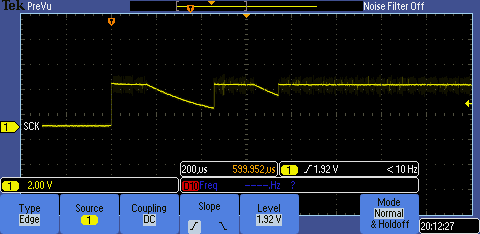
\includegraphics[width=0.7\textwidth]{images/debon_LtoH.png}
		\caption{Signal from switch. Low to high}
	\end{centering}
\end{figure}
From the figure above it is clear that the switch is bouncing, and it is possible to see how long it takes the switch to be stable. From the measurements it takes around $750\mu s$.
\begin{figure}[H]
	\begin{centering}
		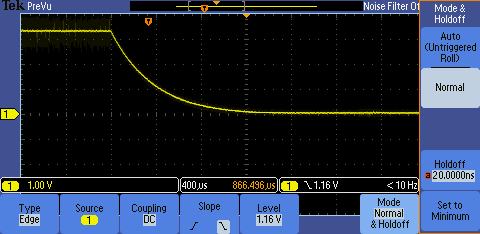
\includegraphics[width=0.7\textwidth]{images/debon_HtoL.png}
		\caption{Signal from switch. High to low}
	\end{centering}
\end{figure}
The figure above shows the switch signal from high to low, this signal is now bouncing, and would not cause any problem because the slope is negative at all time, so when the signal hits the point where the Spartan 6 is switching, the signal would not trigger a switch back. But is takes around $1200\mu s$ for the switch to stabilise.
\subsubsection{Design}
%       	 Design
%
%                UML/SysML deployment view(s)
%                Mechanical specifications and dimensioning
%                HW module specification per block
%                UML SW deployment view
%                Class specification
%                Refactored class diagram
%                Use case scenarios specifications
%                Sequence diagrams
%
In order to remove any debouncing on the switches, a delay is needed. In this system the time has to be the double plus one bit. From the measurements the longest time is $1200\mu s$, the double of that is $2400\mu s$. Calculations for the delay is shown below.
\begin{align}
	t &=	1200\mu s \cdot 2 \\
	f &=	100MHz\\
	t &=	2^{n}\cdot \dfrac{1}{f}\\
	n &=	\dfrac{\ln(f\cdot t)}{\ln(2)}\\
	n &=	\dfrac{\ln(100MHz\cdot 2400\mu s)}{\ln(2)}\\
	n &=	17.87
\end{align}
The bit length for the double delay is 18 and plus 1 bit, a 19 bit vector has to be used in the delay. The delay for 19 bit vector is.
\begin{align}
	t &=	2^{19}\cdot \dfrac{1}{100MHz}\\
	t &=	5.243 ms\\
\end{align}
This is the time delay that is used to debounce the switches.
\subsubsection{Conclusion}
This time delay has been tested in timebox 6 and it is working with the interrupt register in the Spartan 6.
%
%
%
% % % % % % % % % % % % % % % % % % % % % % % % % % % % % % % % % % % % % % % % %
\subsection{Verification - Theis}
%			Intro
%					verification specification
%					deployment specification
%
From the former timeboxes the blocks in the Spartan 6 has been implemented to make a complete system, which is communicating with the external memory controller in the LPC2478.
\subsubsection{External memory controller}
The EMC interface has been analysed with timings and signal assignment in order to make the Spartan 6 read and write data on the right time. On the figure below a block diagram for the EMC in the LPC2478 is shown. The data and pictures is taken from the \textit{LPC24xx user manual}\footnote{\url{http://www.nxp.com/documents/user\_manual/UM10237.pdf}} and the \textit{electrical datasheet}\footnote{\url{http://www.nxp.com/documents/data\_sheet/LPC2478.pdf}} for the LPC2478
\begin{figure}[H]
	\begin{centering}
		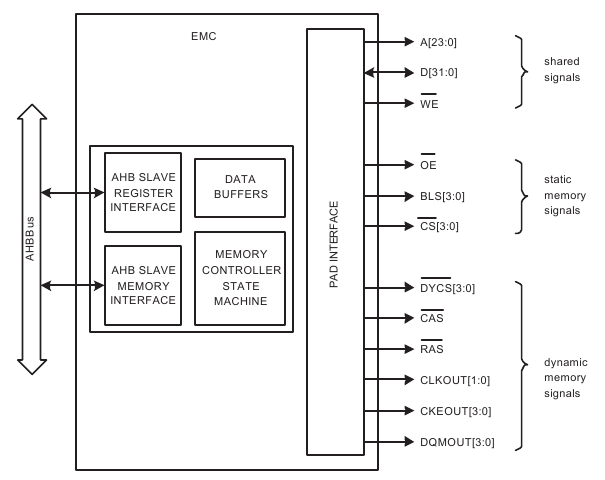
\includegraphics[width=0.8\textwidth]{images/tb7_EMC_block.png}
		\caption{EMC block}
	\end{centering}
\end{figure}
The EMC is used in static mode without the \textit{BLS}\footnote{Byte lane selects} signal, and for memory selection it is only using the \textit{CS2}\footnote{Chip Select 2} for the Spartan 6, this is the interface that has to be implemented in the Spartan 6 to control the wishbone master. The block that takes care of this assignment is the host controller from timebox 3. The timings and signal assignment is shown on the next to figures.
\begin{figure}[H]
	\begin{centering}
		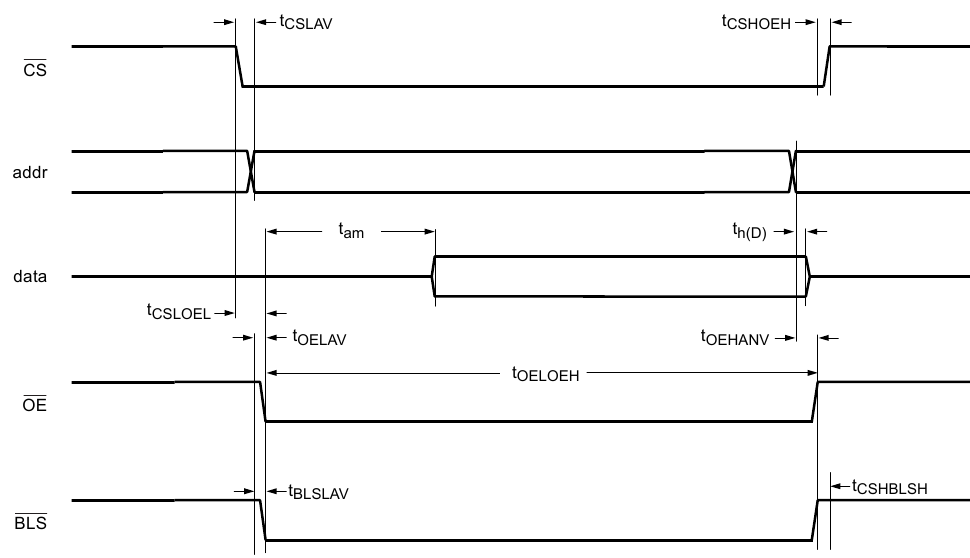
\includegraphics[width=0.8\textwidth]{images/tb7_EMC_read.png}
		\caption{EMC Read timing}
	\end{centering}
\end{figure}
The important thing when the EMC read data from the Spartan 6, is the $t_{am}$ this is where the EMC reads the data from the Spartan 6, therefore the Spartan 6 has to have valid data ready latest at that time, for the EMC to read correct data. From the electrical datasheet the timing for $t_{am}$ is taken.
\begin{align}
t_{am}min &= (WAITRD - WAITOEN + 1) \cdot T_{cy} - 12.70ns\\
t_{am}typ &= (WAITRD - WAITOEN + 1) \cdot T_{cy} - 9.57ns\\
t_{am}max &= (WAITRD - WAITOEN + 1) \cdot T_{cy} - 8.11ns
\end{align}
The \textit{WAITRD} and \textit{WAITOEN} is integer values that is set in the setup of the EMC in the LPC2478, \textit{WAITRD} has influence on the timing of $t_{am}$ and \textit{OELOEH} increasing this value increase the timing. When \textit{WAITOEN} is increased \textit{CSLOEL} is increased to and $t_{am}$ and \textit{OELOEH} is decreased. The $T_{cy}$ is the time of the clock period.
\begin{align}
CCLK &= 72MHz\\
T_{cy} &= \dfrac{1}{CCLK}\\
T_{cy} &= 13.889ns
\end{align}
The exact timing of $t_{am}$ is calculated late with the Bus functional module used for verification of the Spartan 6 design.
\begin{figure}[H]
	\begin{centering}
		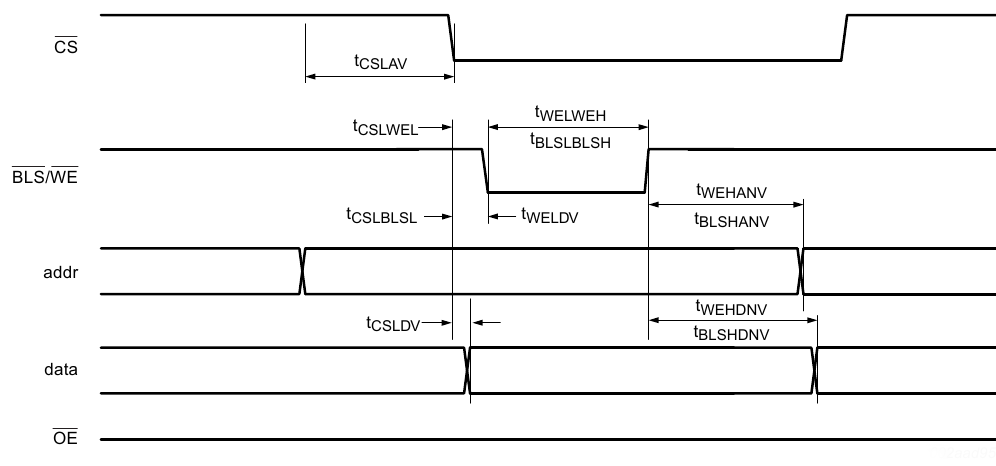
\includegraphics[width=0.8\textwidth]{images/tb7_EMC_write.png}
		\caption{EMC Write timing}
	\end{centering}
\end{figure}
The write diagram shows that the data is valid at the same time as \textit{WE}\footnote{Write Enable} is set low, as long as the Spartan 6 is reacting on \textit{CS2} and the \textit{WE} invalid data is not a problem.
\subsubsection{Bus functional module}
The bus functional module is a module written in VHDL for test purpose. A BFM is able to simulate different interfaces, depending on the code. In this project the BFM is used to test the total design of the Spartan 6 by simulating the EMC interface from the LPC2478. A rough code sketch was handed out from Morten Opprud Jakobsen, timing tweaks needed to be updated in order to make a correct simulation.\\
\dirtree{%
.1 \textcolor{blue}{sim}. 
.2 arm\_emc\_package.vhd. 
.2 \textcolor{blue}{log}. 
.3 arm7\_bfm\_log.txt. 
.2 \textcolor{blue}{stim}. 
.3 arm7\_bfm\_stim.dat. 
.2 tb\_ARM\_BFM.vhd. 
.2 txt\_util.vhd\\. 
}
The file structure of the BFM is shown above, in \textit{arm\_emc\_package.vhd} all the timings and constants is contained. This file also holds the functions for a read and write cycle, with signal assignment in the correct order and time from the timings. \textit{txt\_util.vhd} holds function for converting text strings. The \textit{tb\_ARM\_BFM.vhd} is the test bench file, this file takes a data input from the data file. The data file tells the BFM what to do, if it shall read, write, wait or log something, the logs is written to the log file. The BFM is used on the final Spartan 6 design with the following data file.
\begin{lstlisting}[caption=BFM data file]
#WAIT 10
#LOG Write 0x00 to LEDs
#WR 0000000000010000 0000000000000000
#LOG Change switches
#SW 01000000
#WAIT 30
#LOG Read IRQ reg
#RD 0000000000000000
#LOG Read switch reg
#RD 0000000000100000
#LOG Write 0x00 to LEDs
#WR 0000000000010000 0000000001000000
#WAIT 10
#END
\end{lstlisting}
The test bench signals is shown below. In the first figure, the BFM write to the LEDs to turn off, in the figure it is shown that the LEDs is changed to all zeros. Next the switches positions is changed, the arrow shows that the interrupt to the LPC2478 is activated after the switches is changed.
\begin{figure}[H]
	\begin{centering}
		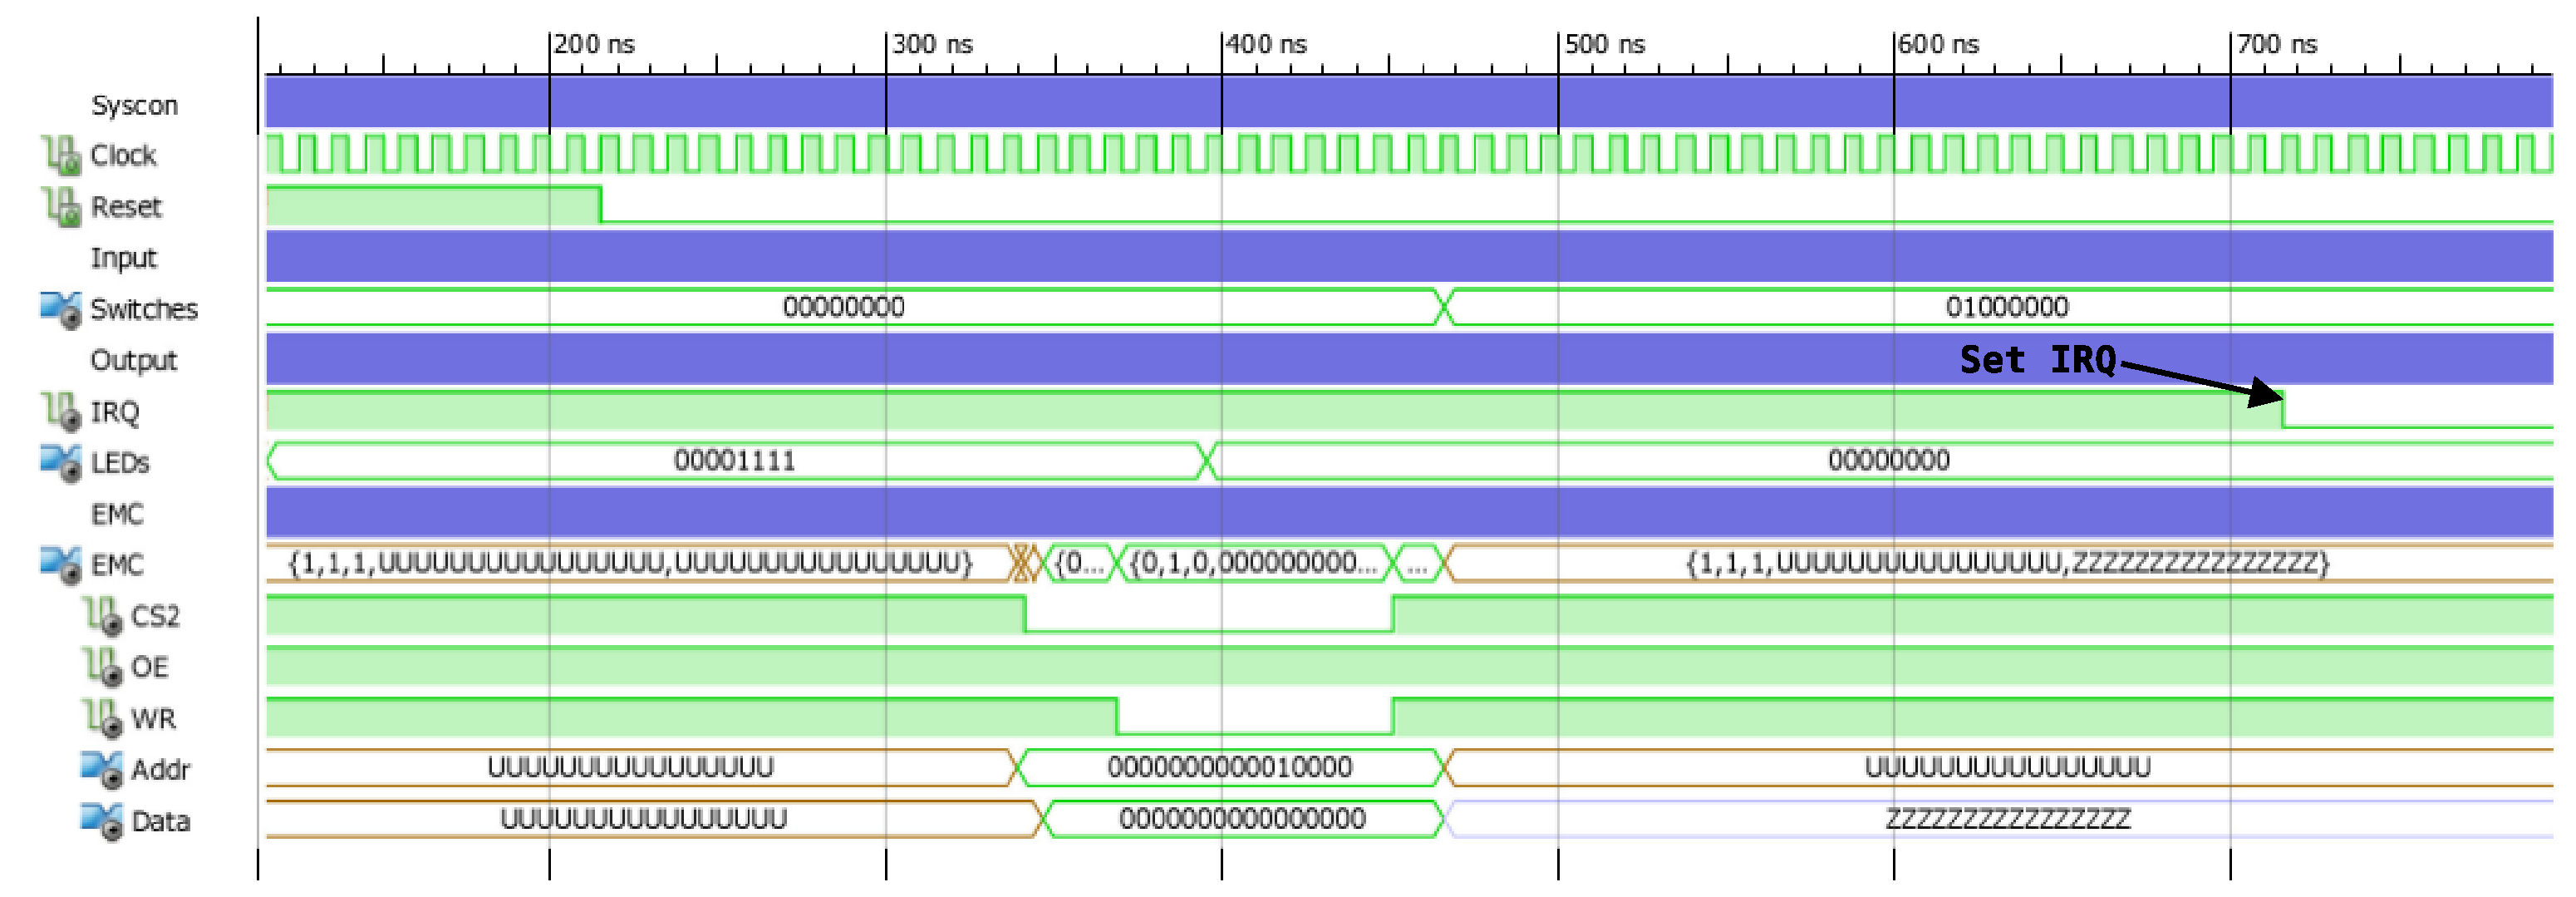
\includegraphics[width=1.0\textwidth]{images/tb7_BFM_write.eps}
		\caption{BFM write}
	\end{centering}
\end{figure}
The figure below is the continued BFM test bench. First the BFM reads the interrupt register, the first arrow shows when the data is valid on the Spartan 6, the blue maker indicate when the EMC is reading data from the Spartan 6. The second arrow shows that the interrupt is deactivated as the interrupt register is read. Next the BFM read the switch register to get the switch position, the arrow again shows when the data is valid, and the blue marker show when the data is read. Last the LEDs is set to the new switch position by another write to the LEDs from the BFM.
\begin{figure}[H]
	\begin{centering}
		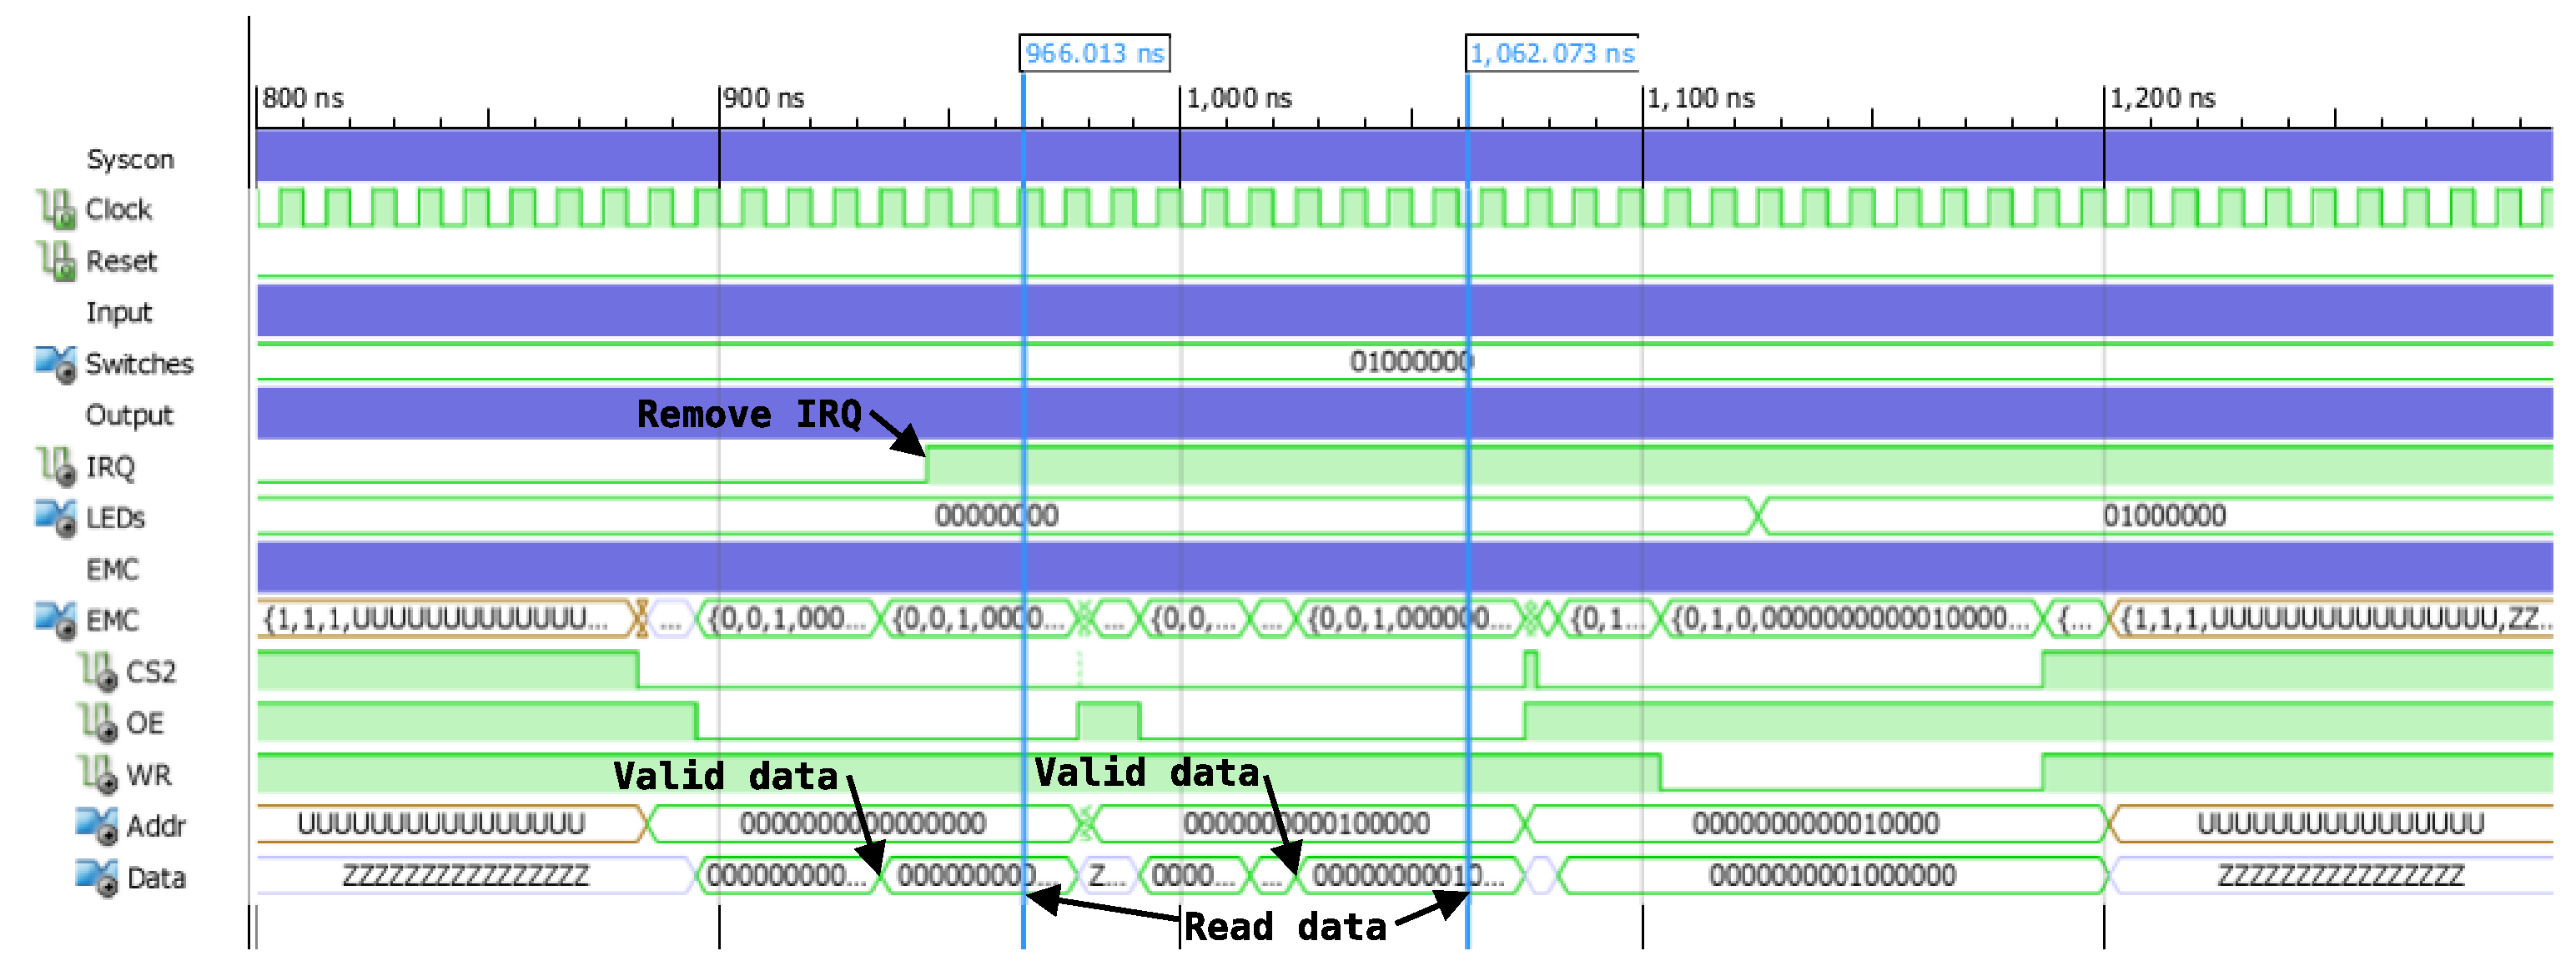
\includegraphics[width=1.0\textwidth]{images/tb7_BFM_read_irq.eps}
		\caption{BFM read IRQ}
	\end{centering}
\end{figure}
\subsubsection{Digital clock manager}
In the code handed out by Morten Opprud Jakobsen, there is a DCM\footnote{Digital Clock Manager}. This module is used for making a jitter-free clock, and have the possibility to change the clock speed in order to match the clock for the LCP2478. The DCM in Spartan 6 tolerates two types of jitter, \textit{cycle-to-cycle jitter} and \textit{period jitter}. Cycle-to-cycle jitter is the change in clock period from cycle to cycle, the period jitter is the change over millions of clock cycles. The code for the DCM is shown below.
\begin{lstlisting}[language=VHDL, caption=DCM\_SP]
...
	clk_o <= clk_r;

-- DCM instantiation for the system clock.
	DCM_Sys : DCM_SP
	generic map (
		CLKFX_DIVIDE				=> 2,											-- Can be any integer from 1 to 32
		CLKFX_MULTIPLY			=> 2)											-- Can be any integer from 2 to 32
	port map	(
				CLK0				=> clk_s,											-- 0 degree DCM CLK ouptput
				CLKFX				=> clk_r,											-- DCM CLK synthesis out (M/D)
				CLKFB				=> clk_s,											-- DCM clock feedback
				CLKIN				=> clk_i,											-- Clock input (from IBUFG, BUFG or DCM)
				RST					=> '0'												-- DCM asynchronous reset input
				);
...
\end{lstlisting}
The DCM in the Spartan 6 has many different features, one of the features that is used is removing jitter, this is done in the code above. The DCM takes the standard clock input, and the zero phase shifted clock is routed into the clock feedback, for the DCM to compensate for jitter. The DCM is also used to scale the clock to match the clock in the LPC2478, this is done by multiplying and dividing the clock with integer values.
\subsubsection{Spartan 6}
The final design of the Spartan 6 in this project has been verified and the figure below shows the top layer block, and the inputs and outputs on the Spartan 6.
\begin{figure}[H]
	\begin{centering}
		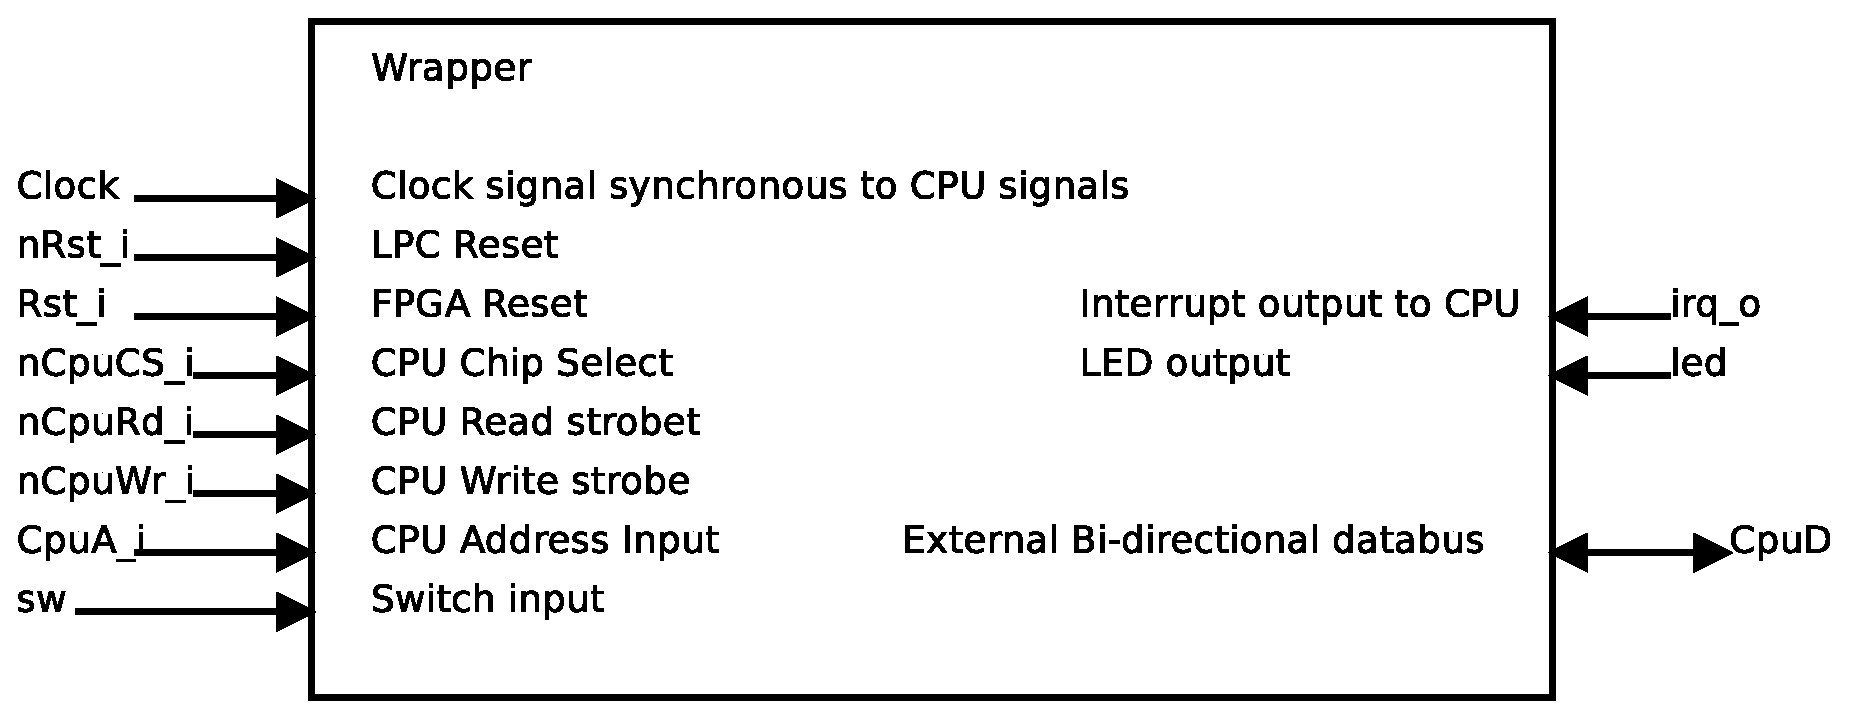
\includegraphics[width=0.9\textwidth]{images/tb7_wrapperblock.eps}
		\caption{Top level in Spartan 6}
	\end{centering}
\end{figure}
The Spartan 6 acts as a memory block seen from the EMC in the LPC2478, the memory map for the Spartan 6 is shown below, with slave addresses, data direction and data length.
\begin{table}[H]
    \begin{tabular}{|l|l|l|l|l|l|p{3.7cm}|}
        \hline
        Name         & DIR		 & S select 	& S address 	& Data                & EMC address & Note                                  \\ \hline
        IRQ Register & Read      & 000          & 0000          & 7 bit - 6 down to 0 & 0x82000000        & Hold data from the interrupting slave \\ \hline
        LED          & Write     & 001          & 0000          & 8 bit - 7 down to 0 & 0x82000020        & Set states of LEDs                    \\ \hline
        Switch       & Read      & 010          & 0000          & 8 bit - 7 down to 0 & 0x82000040        & Hold state of switches                \\
        \hline
    \end{tabular}
    \caption{Memory map of Spartan 6\\
    		 S = Slave, DIR = Direction}
\end{table}
\subsubsection{Conclusion}
The BFM verify the design, and it has been tested on the hardware and it is working properly. It is not possible to measure the clock speed with the equipment at the university, so it is not possible to verify that the code fails without the DCM because of jitter on the clock.
% % % % % % % % % % % % % % % % % % % % % % % % % % % % % % % % % % % % % % % % %
% % % % % % % % % % % % % % % % % % % % % % % % % % % % % % % % % % % % % % % % %
% Jesus Thing
% % % % % % % % % % % % % % % % % % % % % % % % % % % % % % % % % % % % % % % % %
\subsection{Jesus thing - Paulo}
%			Intro
%					verification specification
%					deployment specification
%
\subsubsection{Analysis}
%			Analysis
%
%                Refactored block diagram
%                Refactored class diagram
%                Detailed use cases
%                User interface specification
%                System interface specification
%                Dimensioning specification 
%
\subsubsection{Design}
%       	 Design
%
%                UML/SysML deployment view(s)
%                Mechanical specifications and dimensioning
%                HW module specification per block
%                UML SW deployment view
%                Class specification
%                Refactored class diagram
%                Use case scenarios specifications
%                Sequence diagrams
%
\subsubsection{Implementation}
%     	   Implementation
%
%                Mechanical drawings with details explained
%                Electronic diagrams with details explained
%                Source code with details explained
%                Description of integration 
%
\subsubsection{Verification}
%       	 Verification
%
%                Module tests
%                Integration tests
%                Acceptance test
\subsubsection{Conclusion}
% % % % % % % % % % % % % % % % % % % % % % % % % % % % % % % % % % % % % % % % %
% % % % % % % % % % % % % % % % % % % % % % % % % % % % % % % % % % % % % % % % %
% Dennis Thing
% % % % % % % % % % % % % % % % % % % % % % % % % % % % % % % % % % % % % % % % %
\subsection{GPIO Device driver - Dennis}
In order to fulfill the requirements shown in table \ref{tab:gpio_req}\footnote{All requirements can be found in the Appendix EEPRO3}, an driver is needed in order to control the GPIO pins on the micro controller. 
\begin{table}[H]
\centering
	\begin{tabular}{|p{1.2cm}|p{2.8cm}|p{8cm}|p{3.5cm}|}
	\hline
	ID		& Requirement		& Description												& Comments\\\hline
	B-2.1	& Over production & Overproduced energy is wasted in a dummy load connected to the hub. & Energy routing is controlled by GPIO's \\\hline
	B-2.2	& Over production & If two or more producers are connected and one can be without, it is stopped. & Energy routing is controlled by GPIO's \\\hline
	B-2.3	& Under production & If there is no overproduction (dummy load is turned off), the grid is con- nected to the power line in case the producers cannot produce enough energy. & Energy routing is controlled by GPIO's \\\hline
	\end{tabular}
	\caption{Requirements that concerns GPIO}
	\label{tab:gpio_req}
\end{table}
%			Intro
%					verification specification
%					deployment specification
%
\subsubsection{Analysis}
The kernel is running in an embedded system environment with only known parameters connected to it. Therefore a specific GPIO driver is written to decrease development time compared to if a more generic driver was made.
\p In order to verify a part
\begin{table}[H]
	\centering
	\begin{tabular}{|p{2cm}|p{2cm}|p{3cm}|p{3cm}|}\hline
		GPIO nr.		& Pin nr.		& Name			& Direction		\\\hline
		GPIO0		& 0.12		& PLC\_nReset		& Output			\\\hline
		GPIO1		& 0.13		& PLC\_wake		& Output			\\\hline
		GPIO2		& 0.18		& PLC\_nSleep		& Output			\\\hline
		GPIO3		& 2.10		& FPGA\_int		& Input Interrupt	\\\hline
		GPIO4		& 1.6			& PS\_main		& Output			\\\hline
		GPIO5		& 1.23		& PS1\_in			& Output			\\\hline
		GPIO6		& 1.25		& PS2\_in			& Output			\\\hline
		GPIO7		& 1.19		& PS1\_out		& Output			\\\hline
		GPIO8		& 1.21		& PS2\_out		& Output			\\\hline
	\end{tabular}
	\caption{GPIO connection table}
	\label{tab:gpio_table}
\end{table}
Table \ref{tab:gpio_table} shows that there will be one device driver with nine valid minor number calls in it. Each of the GPIO devices identifies a GPIO port on the micro controller. The name is an indication of what the GPIO pin is connected to. 
\p \textit{PLC\_nReset}, \textit{PLC\_wake} and \textit{PLC\_nSleep} controls the Power Line Module, by resetting it, wakening it or put it to sleep when there is no need for it.
\p \textit{FPGA\_int} indicates if the FPGA has new data for the micro controller to read, this is indicated by an interrupt.
\p \textit{PS\_main} Turns on or off the supply from the grid.
\p \textit{PS1\_in} and \textit{PS2\_in} sets each of their power switches as an input port whereas \textit{PS1\_out} and \textit{PS2\_out} sets each of their power switch as an output device.        
%			Analysis
%
%                Refactored block diagram
%                Refactored class diagram
%                Detailed use cases
%                User interface specification
%                System interface specification
%                Dimensioning specification 
%
\subsubsection{Design}
When inserting the module the pins needed are configured and given default values. The driver is made so that the pins can be accessed singly and thereby be given a logical value '0' or '1', or a logical value can be read from a single pin.
\p In order to verify if the GPIO device driver works as excepted, the \textit{echo} command and the \textit{cat} commands have been used.
\\ Example of reading GPIO0: \textit{cat /dev/gpio0}
\\ Example of setting GPIO0 to 1: \textit{echo 1 /dev/gpio0}
\p In order to control the power switches an user space application has been written to easy the control of these. The program reads the two first arguments of argv. argv[1] defines the power switch to control, where 0 controls GPIO4 which is the power switch controlling the main. 1 and 2 each controls a power switch connected to a module (wind turbine, battery or similar). argv[2] defines the action of the power switch, where valid arguments are: \textit{in}, \textit{out} and \textit{off}.
\begin{itemize}
	\item in, opens for energy flow from a module to the power line.
	\item out, opens for energy flow from the power line to a module.
	\item off, turns off energy flow in both directions.
\end{itemize}
\begin{lstlisting}[language=c, caption=User space application to control the Power switches]
/*
 ============================================================================
 Name        : port.c
 Author      : E10-Team3 dENNES
 Description : EA-LPC2478 - Control of the power switches connected
 ============================================================================
 */
#define GPIO "/dev/gpio"

/*
        PORT <num> <status>

        Status: in, out, off
        num: 0, 1, 2
        
        in      out
----------------------------
        4       x               PORT0
        5       7               PORT1
        6       8               PORT2
----------------------------
*/


int main(int argc, char *argv[]) {
        	int fd, ret, num;
        	char ibuff[10], obuff[10];
        	char val;	
	char *cmd;
	char dev[3][2]

	num = *argv[1]-'0';
	cmd = argv[2];

        	if(num >= 0 && num <= 2){		// Check if a valid port is called
         		if(strncmp("in", cmd, 2) == 0){	// Set module as input
                   	printf("\nINPUT port%d",num);
                        	dev[num][0] = '1';
                        	dev[num][1] = '0';
                	}
                	else if(strncmp("out", cmd, 3) == 0){	// Set module as output
                       	printf("\nOUTPUT");
                        	dev[num][0] = '0';
                        	dev[num][1] = '1';
                	}
                	else if(strncmp("off", cmd, 3) == 0){	// Turn off module in both directions
                        	dev[num][0] = '0';
                        	dev[num][1] = '0';
                	}
                	else{							// Invalid command sent
                        	printf("\nSomething wrong");
                        	exit(-1);
                	}

                	sprintf(ibuff,"%s%d",GPIO,num+4);	// Compress write string
                	sprintf(obuff,"%s%d",GPIO,num+6);	// ex. /dev/gpio4 if PORT0

                	if((fd = open(ibuff,O_WRONLY)) < 0){	// Open GPIO device driver
                        	printf("Cannot open file in.\n");
                        	exit(-1);
                	}
                	ret = write(fd, &dev[num][0], 1);
                	if(ret < 0){
                        	printf("Write failed in: %d\n", ret);
                        	exit(-1);
                	}
                	close(fd);

                	if(num != 0){					// If port 1 or 2, set second pin on module
                        	if((fd = open(obuff,O_WRONLY)) < 0){
                                	printf("Cannot open file out.\n");
                                	exit(-1);
                        	}
                        	ret = write(fd, &dev[num][1], 1);
                        	if(ret < 0){
                                	printf("Write failed out: %d\n", ret);
                                	exit(-1);
                        	}
                	close(fd);
                	}
        	}
        	return 0;
}
\end{lstlisting}


%       	 Design
%
%                UML/SysML deployment view(s)
%                Mechanical specifications and dimensioning
%                HW module specification per block
%                UML SW deployment view
%                Class specification
%                Refactored class diagram
%                Use case scenarios specifications
%                Sequence diagrams
%
\subsubsection{Implementation}

The gpio header file contains prototypes of the functions used, defines and arrays holding values for the different registers to call in order to avoid \textit{if/else} or \textit{switch/case} in the different functions. 
\begin{lstlisting}[language=c, caption=GPIO header file ]
#define GPIO_MAJOR 245
#define NUM_GPIO_DEVICES 9

#define GPIO_IRQ 14
---
static u32 fdir[] ={
	FIO0DIR,
	FIO0DIR,
	FIO0DIR,
	FIO2DIR,
	FIO1DIR,
	FIO1DIR,
	FIO1DIR,
	FIO1DIR,
	FIO1DIR,
};
---
\end{lstlisting}
The fops (file operations structure) structure with the different device driver call possibilities. This device driver can be opened, closed, read and write.
\begin{lstlisting}[language=c, caption=GPIO fops structure]
static struct file_operations gpio_fops = {
	.owner   	= THIS_MODULE,
	.read			= gpio_read,
	.write  	= gpio_write,
	.open    	= gpio_open,
	.release	= gpio_close,
};
\end{lstlisting}
Initialization of the GPIO pins is called from the init function. The \textit{init} and \textit{exit} functions are similar to the once implemented in the ADC and the UART device drivers except for the \textit{gpioInit} function call.
\begin{lstlisting}[language=c, caption=GPIO init function]
static void gpioInit(void){
	int i=0;
	m_reg_bfs(SCS, 0x1);	// Enable fast I/O on port 0 and 1
	for(i=0 ; i<NUM_GPIO_DEVICES ; i++){
		m_reg_bfc(psel[i], enable_pinsel[i]);
		if(i != 3){
			m_reg_bfs(fdir[i], gpio_pins[i]);
			m_reg_bfs(pin_default_reg[i], gpio_pins[i]);
		}
	}
}
\end{lstlisting}
When the file is opened, the interrupt is configured if it is GPIO3 that is called.
\begin{lstlisting}[language=c, caption=GPIO open function]
static int gpio_open(struct inode* inode, struct file* file){
---
	if(num == 3){
		// setup interrupt for pin input
		DPRINT("\nEnable int for input");
		flag = 0;
		m_reg_bfs(EXTMODE, 1);		// INT0 Edge sensitive
		m_reg_bfc(EXTPOLAR, 1);		// falling edge 
		m_reg_bfs(EXTINT, 1);			// clear pending INT0 interrupts

		ret = request_irq(GPIO_IRQ, interrupt_gpio, SA_INTERRUPT,"GPIO P2.10 interrupt", NULL);
					//SA_SHIRQ 	= Shared interrupt
					//SA_INTERRUPT 	= Fast interrupt

		if(ret){
			printk("IRQ%d is not free. RET: %d\n", GPIO_IRQ, ret);		
			return ret;
		}
	}
	return 0;
}
\end{lstlisting}
The interrupt is freed in the close function if operating in the GPIO3 file.
\begin{lstlisting}[language=c, caption=GPIO close function]
static int gpio_close(struct inode* inode, struct file* file){
---
	if(num == 3){
		free_irq(GPIO_IRQ, NULL);
	}

	return 0;
}
\end{lstlisting}
When read the file returns the character '1' or '0' according to which value the output has. If GPIO3 it read '0' is returned if the pin is low, otherwise the driver is sent to sleep until the pin is '0'. GPIO3 is connected to a pin on the FPGA which is used to symbolize that data is ready to be read from it. The pin goes high again after the external memory address \textit{0x82000000} has been read.
\begin{lstlisting}[language=c, caption=GPIO read function]
static ssize_t gpio_read(struct file *p_file, char *p_buf, size_t count, loff_t *p_pos){
---
	if(num == 3){
		if((m_reg_read(pin_read[num]) & gpio_pins[num]) > 0){
			DPRINT("\nNo interrupt from FPGA, SLEEP!\n");
			m_reg_bfs(PINSEL4, (1<<20));				// Set p2.10 to EINT0
			wait_event_interruptible(my_queue, (flag != 0));	// Put the function to sleep		
			flag = 0;
		}
		value[0] = '0';
	}
	else{
		DPRINT("\nREAD ELSE");
		if((m_reg_read(pin_read[num]) & gpio_pins[num]) > 0){
			value[0] = '1';
		}
		else{
			value[0] = '0';
		}
	}

	if(copy_to_user(p_buf, value, count)){	// Copy read value to user space
		DPRINT("\nFailed: copy_to_user");
		return -EFAULT;
	}
	return 1;
}
\end{lstlisting}
The value written to the device driver shall be a logical '0' or '1' which is then set on the appropriate GPIO pin.
\begin{lstlisting}[language=c, caption=GPIO write function]
static ssize_t gpio_write(struct file *filp, const char *bufp, size_t count, loff_t *p_pos){
---
	if(copy_from_user(value, bufp, count)){	// Copy value from user space to kernel space
		return -EFAULT;
	}
	if(value[0] == '0'){
		//FIO_CLEAR
		DPRINT("\nCLEAR PIN");
		m_reg_bfs(pin_clear[num], gpio_pins[num]);
	}
	else if(value[0] == '1'){
		//FIO_SET
		DPRINT("\nSET PIN");
		m_reg_bfs(pin_set[num], gpio_pins[num]);
	}
	else{
		DPRINT("\nNot a valid character");
		return -EFAULT;
	}

	return count;
}
\end{lstlisting}
If the driver is sent to sleep (in the read function) it jumps to the \textit{interrupt\_gpio} function when awakened as result of the pin having a falling edge.
\begin{lstlisting}[language=c, caption=GPIO interrupt function for GPIO3]
static irqreturn_t interrupt_gpio(int irq, void *dev_id){
	
//	cread = m_reg_read(urbr[0]);		// Read the buffer
	
	DPRINT("\nREAD int\n");	

	m_reg_bfs(EXTINT, 1);		// clear pending INT0 interrupts
	flag = 1;
	wake_up_interruptible(&my_queue);
	return IRQ_HANDLED;
}
\end{lstlisting}

%     	   Implementation
%
%                Mechanical drawings with details explained
%                Electronic diagrams with details explained
%                Source code with details explained
%                Description of integration 
%
\subsubsection{Verification}
In order to test requirement B-2.1, B-2.2 and B-2.3 the whole system needs to be assembled. Table \ref{tab:gpio_req_test} shows the tests described in the Launch phase. 
\begin{table}[H]
\centering
	\begin{tabular}{|p{1.0cm}|p{3.0cm}|p{9.0cm}|p{2.5cm}|}
	\hline
	ID		& Requirement		& Test Description		& Grade/Comment\\\hline
	B-2.1	& Energy Control - Over-Production & A dummy load and a producing module is connected to the system. As no consumers is connected, the system is over- producing. The current flow to the dummy load is measured. If the current flowing to the dummy load is the same as the one coming from the producer (maximum -10\%), the test is valid. &~\\\hline
	B-2.2	& Energy Control - Under-Production & A dummy load and a producing module is connected to the system. As no consumers is connected, the system is over- producing. A variable consuming module is now connected. The resistance in the consuming module is decreased (increas- ing load). The current flow to the dummy load shall now fall. When no current is flowing to the dummy load, it shall be ob- served that the grid is connected. This is done by increasing the load of the consuming module and measuring the current flow from the grid. &~\\\hline
	\end{tabular}
	\caption{Verification of energy routing requirements.}
	\label{tab:gpio_req_test}
\end{table}
As these tests cannot be performed, due to only a part of the system is finish, a minor test has been made in order to verify the functionality of the written device driver.
\p With a multimeter the different pins used as outputs are measured one by one and the output set by sending a value to the file by the \textit{echo} command. Also the pins are read with the \textit{cat} command after setting the pin in order to verify the read function.
\p The interrupt input pin is tested by reading the pin when the FPGA is not yet interrupting to verify if it goes to sleep. If the interrupt pin are read after an interrupt has been given from the FPGA, '0' is returned. 

%       	 Verification
%
%                Module tests
%                Integration tests
%                Acceptance test
\subsubsection{Conclusion}
The small GPIO device driver test has been made with success. All 8 output pins can be set and cleared through the driver. Also the status of the 8 output pins and the one input pin can be read through the driver. If the FPGA has set the interrupt pin to '0', the driver returns '0' immediately without waiting for an falling edge.
% % % % % % % % % % % % % % % % % % % % % % % % % % % % % % % % % % % % % % % % %
% % % % % % % % % % % % % % % % % % % % % % % % % % % % % % % % % % % % % % % % %
% Deployment
% % % % % % % % % % % % % % % % % % % % % % % % % % % % % % % % % % % % % % % % %
\subsection{Deployment}
	%which versions of the prototype the customer will get
	%with what functionality.
\paragraph{Theis thing}
%
%
\paragraph{Jesus thing}
%
%
\paragraph{GPIO Device driver}
%
%